\chapter{Diagramas binarios líquido--vapor y destilación}\label{ch:b2:liquid-vapour-diagrams}

Un alambique de cobre convierte un vino de pocos grados de alcohol en un aguardiente
varias veces más fuerte; una columna de refinería separa el petróleo crudo en sus fracciones, del gas al
fuelóleo pesado. Ambos se basan en un hecho: el vapor que hay sobre una mezcla en ebullición es
más rico que el líquido en el componente más volátil. Si se repiten la
evaporación y la condensación las veces suficientes, la separación es tan
nítida como se quiera, con una excepción: ninguna destilación, por larga que sea la
columna, lleva el etanol más allá de un 95 por ciento en masa aproximadamente. Este capítulo traza
los diagramas que dicen cómo hierve una mezcla de dos líquidos, y los usa para
diseñar una columna y ver dónde debe detenerse.

\begin{recall}
\Cref{ch:b2:chemical-potential}: el \omterm{def:b2:chemical-potential:chemical-potential}{potencial químico}, la \omterm{thm:b2:chemical-potential:raoult}{ley de Raoult} y la
\omterm{def:b2:chemical-potential:ideal-mixture}{mezcla ideal}, los \omterm{def:b2:chemical-potential:activity-coefficient}{coeficientes de actividad} y las desviaciones respecto de la \omterm{thm:b2:chemical-potential:raoult}{ley de Raoult}, la
relación de Gibbs--Duhem. \Cref{ch:b2:equilibrium-shifts}: la \omterm{def:b2:equilibrium-shifts:variance}{varianza}. El
volumen del primer año, sobre técnicas de laboratorio: la destilación simple, los líquidos miscibles e
inmiscibles. El volumen escolar: la destilación y la hidrodestilación.
\end{recall}

\begin{omfigure}
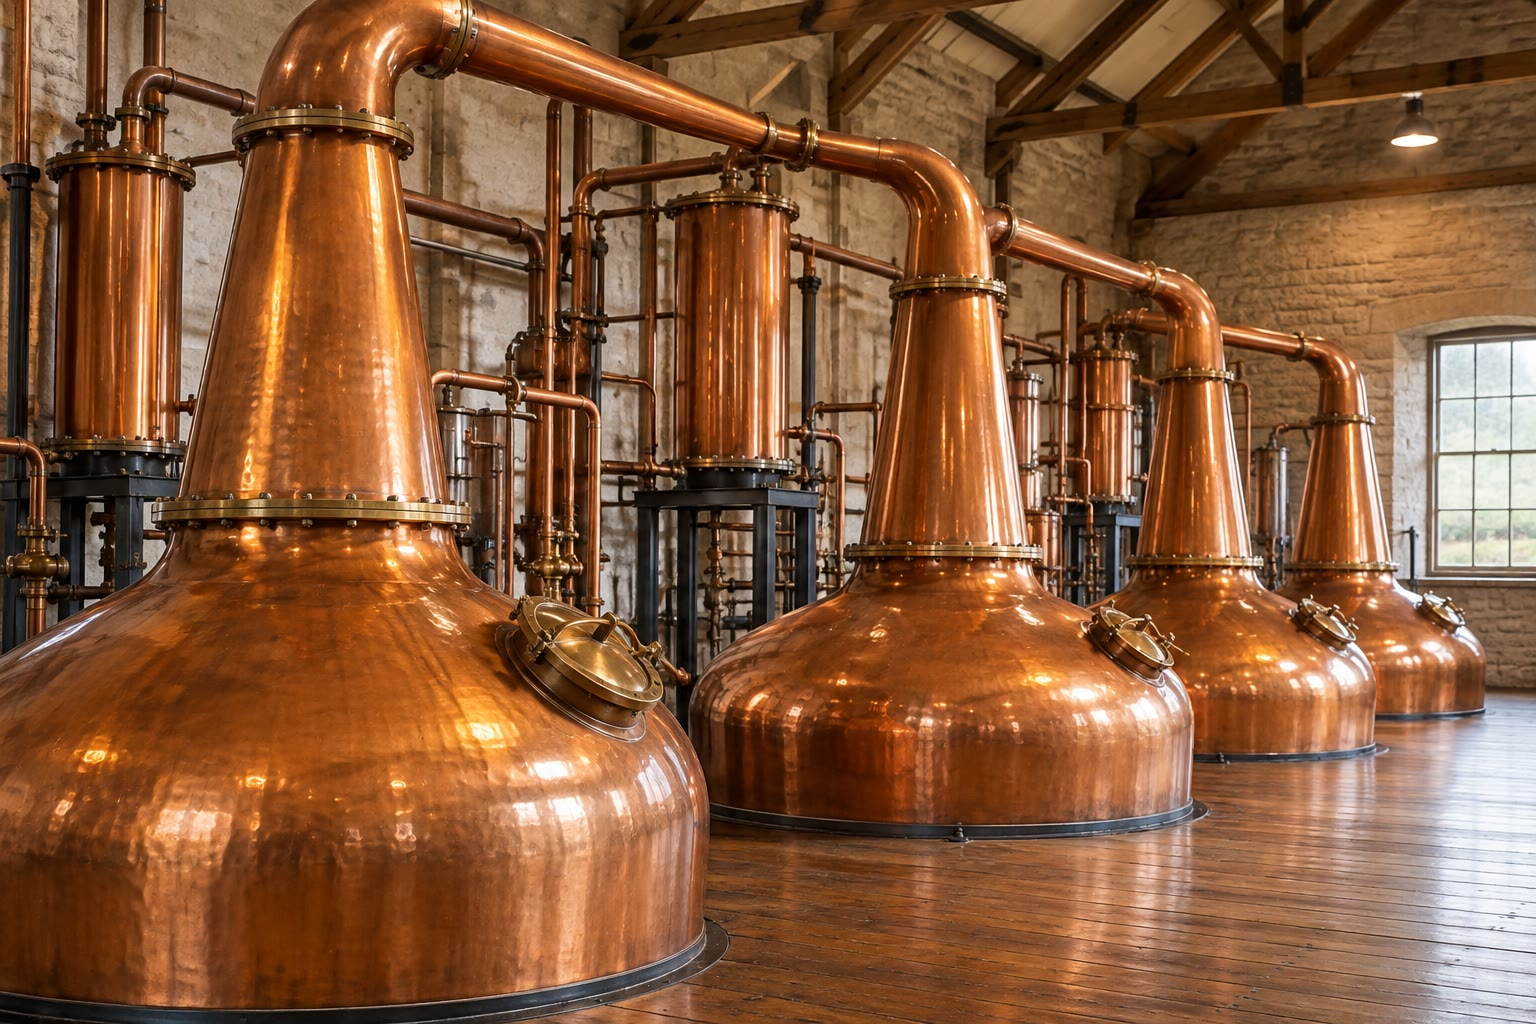
\includegraphics[width=0.62\linewidth]{images/book3/ai/b2-07-pot-stills.jpg}

{\small Alambiques de cobre en una destilería. Cada carga de mosto fermentado se
lleva a ebullición y su vapor se condensa: el primer destilado es varias veces más rico
en etanol que el mosto, y una segunda destilación lo concentra aún más.}
\end{omfigure}

\section{Mezclas ideales}

En este capítulo los dos líquidos se numeran 1 (el más volátil, de menor
punto de ebullición) y 2; $x$ es la fracción molar de 1 en el líquido, e $y$ su
fracción molar en el vapor, que se trata como un gas ideal.

\begin{definition}[Diagrama binario]\label{def:b2:liquid-vapour-diagrams:binary-diagram}
Un \emph{diagrama binario}\index{diagrama binario} indica, para una mezcla de dos
componentes, qué fases están presentes y con qué composiciones, en
función de la composición global y de otra variable. Un
\emph{diagrama isobárico}\index{diagrama isobarico@diagrama isobárico} se traza en el plano
(composición, temperatura) a presión fija; un \emph{diagrama
isotermo}\index{diagrama isotermo}, en el plano (composición, presión) a
temperatura fija.
\end{definition}

\begin{definition}[Curvas de burbuja y de rocío]\label{def:b2:liquid-vapour-diagrams:bubble-dew}
En un diagrama líquido--vapor, la \emph{curva de burbuja}\index{curva de burbuja} da
la composición del líquido en equilibrio con el vapor, y la \emph{curva de
rocío}\index{curva de rocio@curva de rocío}, la del vapor en equilibrio con el líquido. Para una
mezcla de composición dada a presión fija, el \emph{punto de
burbuja}\index{punto de burbuja} es la temperatura a la que aparece la primera burbuja de
vapor al calentar, y el \emph{punto de rocío}\index{punto de rocio@punto de rocío}, la
temperatura a la que aparece la primera gota de líquido al enfriar el vapor.
\end{definition}

\begin{proposition}[Curvas ideales]\label{prop:b2:liquid-vapour-diagrams:ideal-curves}
Para una \omterm{def:b2:chemical-potential:ideal-mixture}{mezcla ideal} a la temperatura $T$, siendo $p_1^*$ y $p_2^*$ las presiones de vapor
de los líquidos puros, la \omterm{def:b2:liquid-vapour-diagrams:bubble-dew}{curva de burbuja} del \omterm{def:b2:liquid-vapour-diagrams:binary-diagram}{diagrama isotermo} es
la recta $p = p_2^* + x(p_1^* - p_2^*)$, y la \omterm{def:b2:liquid-vapour-diagrams:bubble-dew}{curva de rocío} es la
hipérbola
\[
  p = \frac{1}{y/p_1^* + (1 - y)/p_2^*} .
\]
\end{proposition}

\begin{proof}
La \omterm{thm:b2:chemical-potential:raoult}{ley de Raoult} da las presiones parciales $p_1 = xp_1^*$ y $p_2 = (1 -
x)p_2^*$; su suma es la presión total, lineal en $x$. En el vapor,
$y = p_1/p$, luego $x = yp/p_1^*$ y $1 - x = (1 - y)p/p_2^*$; sumando,
$1 = p\,[y/p_1^* + (1 - y)/p_2^*]$.
\end{proof}

\begin{proposition}[El vapor es más rico en el componente más volátil]\label{prop:b2:liquid-vapour-diagrams:richer}
Para una \omterm{def:b2:chemical-potential:ideal-mixture}{mezcla ideal} con $p_1^* > p_2^*$ y $0 < x < 1$, $y > x$.
\end{proposition}

\begin{proof}
$y = xp_1^*/p$ con $p = xp_1^* + (1 - x)p_2^* < p_1^*$, ya que $p$ es una
media ponderada de $p_1^*$ y $p_2^*$, estrictamente comprendida entre ambas. Por tanto, $y >
x$.
\end{proof}

El \omterm{def:b2:liquid-vapour-diagrams:binary-diagram}{diagrama isobárico} es el que describe una destilación, que se lleva a cabo a
presión atmosférica. No tiene fórmula sencilla: para cada temperatura entre
los dos puntos de ebullición se calculan $p_1^*(T)$ y $p_2^*(T)$ (aquí con la
ecuación de Antoine, $\log_{10}(p^*/\unit{bar}) = A - B/(T + C)$, ajustada a
presiones de vapor medidas), y después las composiciones del líquido y del vapor que
dan una presión total de \qty{1.013}{bar}:
\[
  x = \frac{p - p_2^*(T)}{p_1^*(T) - p_2^*(T)}, \qquad y = \frac{x\,p_1^*(T)}{p} .
\]
La \omterm{def:b2:liquid-vapour-diagrams:bubble-dew}{curva de burbuja} ya no es recta; la \omterm{def:b2:liquid-vapour-diagrams:bubble-dew}{curva de rocío} sigue estando por encima,
y el vapor sigue siendo más rico en el componente ligero.

\begin{example}[Benceno y tolueno a \qty{90}{\degreeCelsius}]\label{ex:b2:liquid-vapour-diagrams:benzene-toluene}
El benceno y el tolueno forman una mezcla casi ideal. A \qty{90}{\degreeCelsius}
las ecuaciones de Antoine dan $p_1^* = \qty{1.361}{bar}$ (benceno) y $p_2^* =
\qty{0.542}{bar}$ (tolueno). A \qty{1.013}{bar}: $x = (1.013 - 0.542)/(1.361 -
0.542) = 0.575$ e $y = 0.575 \times 1.361/1.013 = 0.773$. Un líquido con un 57.5~\%
de benceno (en moles) hierve a \qty{90}{\degreeCelsius} y da un vapor con un
77~\%.
% ledger: antoine:benzene.A, antoine:benzene.B, antoine:benzene.C, antoine:toluene.A, antoine:toluene.B, antoine:toluene.C
\end{example}

\begin{omfigure}
\begin{tikzpicture}
\begin{axis}[omphase, width=0.47\linewidth, height=6cm, ymin=78, ymax=113,
  xlabel={$x$, $y$ (benceno)}, ylabel={$T$ (\unit{\degreeCelsius})},
  title={\small isobárico, \qty{1.013}{bar}}]
\addplot[omliquidus] table[x=x, y=T] {figdata/out/bachelor-2-liquid-vapour-a.dat};
\addplot[omsolidus] table[x=y, y=T] {figdata/out/bachelor-2-liquid-vapour-a.dat};
\draw[tieline] (axis cs:0.405,95) -- (axis cs:0.626,95);
\fill (axis cs:0.5,95) circle (1.3pt);
\draw[->, thick] (axis cs:0.5,82) -- (axis cs:0.5,104) node[above, font=\scriptsize] {calentamiento};
\node[font=\scriptsize] at (axis cs:0.2,85) {líquido};
\node[font=\scriptsize] at (axis cs:0.85,108) {vapor};
\node[font=\scriptsize, omDef, anchor=north] at (axis cs:0.22,96) {burbuja};
\node[font=\scriptsize, omThm, anchor=south west] at (axis cs:0.62,101) {rocío};
\end{axis}
\end{tikzpicture}\hfill
\begin{tikzpicture}
\begin{axis}[omphase, width=0.47\linewidth, height=6cm, ymin=0.3, ymax=1.1,
  xlabel={$x$, $y$ (benceno)}, ylabel={$p$ (\unit{bar})},
  title={\small isotermo, \qty{80}{\degreeCelsius}}]
\addplot[omliquidus] table[x=x, y=pbub] {figdata/out/bachelor-2-liquid-vapour-b.dat};
\addplot[omsolidus] table[x=x, y=pdew] {figdata/out/bachelor-2-liquid-vapour-b.dat};
\node[font=\scriptsize] at (axis cs:0.75,0.98) {líquido};
\node[font=\scriptsize] at (axis cs:0.2,0.36) {vapor};
\end{axis}
\end{tikzpicture}

{\small Benceno--tolueno, calculado con la \omterm{thm:b2:chemical-potential:raoult}{ley de Raoult} y las ecuaciones de
Antoine. A la izquierda, a presión atmosférica: \omterm{def:b2:liquid-vapour-diagrams:bubble-dew}{curva de burbuja} (azul) y \omterm{def:b2:liquid-vapour-diagrams:bubble-dew}{curva de rocío}
(roja); el líquido de composición 0.5 empieza a hervir a
\qty{92.1}{\degreeCelsius} y está todo vaporizado a \qty{98.8}{\degreeCelsius}; a
\qty{95}{\degreeCelsius} (recta de reparto discontinua) se separa en un líquido de 0.405
y un vapor de 0.626. A la derecha, a \qty{80}{\degreeCelsius}: la \omterm{def:b2:liquid-vapour-diagrams:bubble-dew}{curva de burbuja} es
recta, la \omterm{def:b2:liquid-vapour-diagrams:bubble-dew}{curva de rocío} una hipérbola, y el líquido está ahora arriba.}
% ledger: antoine:benzene.A, antoine:toluene.A (all six parameters in figdata/bachelor-2/liquid-vapour.py)
\end{omfigure}

\section{Lectura de un diagrama}

\begin{proposition}[Varianza de un sistema binario bifásico]\label{prop:b2:liquid-vapour-diagrams:variance}
Una mezcla de dos componentes en dos fases tiene \omterm{def:b2:equilibrium-shifts:variance}{varianza} 2. A presión fija,
la temperatura sola fija las composiciones de ambas fases: se leen
en los extremos del segmento horizontal que pasa por el punto representativo,
llamado recta de reparto.
\end{proposition}

\begin{proof}
Variables intensivas: $T$, $p$, $x$, $y$. Relaciones: igualdad de los \omterm{def:b2:chemical-potential:chemical-potential}{potenciales
químicos} de 1 y de 2 entre las fases. $v = 4 - 2 = 2$ (la regla de las fases
$v = n - r + 2 - \varphi$ da lo mismo con $n = 2$, $r = 0$, $\varphi = 2$).
Fijar $p$ deja un grado de libertad: $x(T)$ e $y(T)$ son las dos curvas.
\end{proof}

\begin{theorem}[Regla de la palanca]\label{thm:b2:liquid-vapour-diagrams:lever}
Una mezcla de composición global $z$, separada en un líquido de composición $x$
y un vapor de composición $y$, contiene cantidades $n_L$ de líquido y $n_V$ de
vapor tales que
\[
  n_L\,(z - x) = n_V\,(y - z), \qquad \frac{n_V}{n_L + n_V} = \frac{z - x}{y - x} .
\]
Es la \emph{regla de la palanca}\index{regla de la palanca}: cada fase es tanto más
abundante cuanto más cerca está su composición de la global, como los pesos de
una palanca que pivota en $z$.
\end{theorem}

\begin{proof}
Conservación del componente 1: $(n_L + n_V)z = n_Lx + n_Vy$, luego $n_L(z - x) =
n_V(y - z)$; se divide por $n_L + n_V$ y se reordena.
\end{proof}

La \omterm{thm:b2:liquid-vapour-diagrams:lever}{regla de la palanca} vale con fracciones molares y cantidades, como aquí, o con fracciones
másicas y masas: la conservación empleada es la misma.

\begin{method}[Leer un diagrama binario]\label{met:b2:liquid-vapour-diagrams:read-diagram}
\begin{enumerate}
  \item Sitúese el punto (composición global, temperatura) y nómbrese su
        dominio: líquido, vapor o líquido + vapor.
  \item En un dominio bifásico, trácese la recta de reparto que pasa por el punto; sus extremos
        dan las composiciones del líquido (sobre la \omterm{def:b2:liquid-vapour-diagrams:bubble-dew}{curva de burbuja}) y del
        vapor (sobre la \omterm{def:b2:liquid-vapour-diagrams:bubble-dew}{curva de rocío}).
  \item Obténganse las proporciones de las fases con la \omterm{thm:b2:liquid-vapour-diagrams:lever}{regla de la palanca}.
  \item Para seguir un calentamiento, desplácese el punto hacia arriba: la primera burbuja aparece
        sobre la \omterm{def:b2:liquid-vapour-diagrams:bubble-dew}{curva de burbuja}, la última gota desaparece sobre la \omterm{def:b2:liquid-vapour-diagrams:bubble-dew}{curva de rocío};
        entre ambas, el líquido se empobrece en el componente ligero.
\end{enumerate}
\end{method}

\begin{example}[Una vaporización súbita a \qty{95}{\degreeCelsius}]\label{ex:b2:liquid-vapour-diagrams:flash}
Se llevan \qty{100}{mol} de una mezcla equimolar de benceno--tolueno a
\qty{95}{\degreeCelsius} a presión atmosférica. La recta de reparto da $x =
0.405$, $y = 0.626$; la fracción de vapor es $(0.500 - 0.405)/(0.626 - 0.405) =
0.43$: \qty{43}{mol} de vapor que contienen $43 \times 0.626 = \qty{27}{mol}$ de
benceno, y \qty{57}{mol} de líquido que contienen \qty{23}{mol}. Una etapa de equilibrio
enriquece, pero solo un poco.
\end{example}

\section{Mezclas reales y azeótropos}

Cuando los \omterm{def:b2:chemical-potential:activity-coefficient}{coeficientes de actividad} difieren de 1 (\cref{ch:b2:chemical-potential}),
las presiones parciales se apartan de las rectas de Raoult. Con una desviación
positiva ($\gamma > 1$: las moléculas distintas se atraen menos que las
iguales) la presión total queda por encima de la recta ideal; con una desviación negativa,
por debajo. Si la desviación es lo bastante fuerte, la presión total pasa por un
extremo.

\begin{definition}[Azeótropo]\label{def:b2:liquid-vapour-diagrams:azeotrope}
Un \emph{azeótropo}\index{azeotropo@azeótropo} es una mezcla líquida que hierve sin
cambiar de composición: el vapor que da tiene su misma composición. Un
\emph{azeótropo positivo}\index{azeotropo positivo@azeótropo positivo} (desviación positiva) presenta
un máximo de presión en el \omterm{def:b2:liquid-vapour-diagrams:binary-diagram}{diagrama isotermo} y un mínimo de temperatura de
ebullición en el isobárico; un \emph{azeótropo negativo}\index{azeotropo negativo@azeótropo negativo},
lo contrario.
\end{definition}

\begin{theorem}[Teorema de Gibbs--Konovalov]\label{thm:b2:liquid-vapour-diagrams:konovalov}
En un \omterm{def:b2:liquid-vapour-diagrams:binary-diagram}{diagrama binario} líquido--vapor, en un extremo de la presión total (a
temperatura fija) o de la temperatura de ebullición (a presión fija), el
líquido y el vapor tienen la misma composición. Recíprocamente, donde las
dos composiciones son iguales, las curvas tienen una tangente horizontal común.
\end{theorem}

\begin{proof}[Demostración a temperatura fija]
La relación de Gibbs--Duhem para el líquido a $T$ fija (despreciando el pequeño efecto de $p$
sobre el líquido) es $x\,d\mu_1 + (1 - x)\,d\mu_2 = 0$. En el equilibrio
$\mu_i = \mu_i^\circ + RT\ln(p_i/p^\circ)$ con $p_1 = yp$, $p_2 = (1 - y)p$, luego
\[
  x\,d\ln(yp) + (1 - x)\,d\ln((1 - y)p) = 0
  \quad\Longrightarrow\quad
  d\ln p = -\Big(\frac{x}{y} - \frac{1 - x}{1 - y}\Big)dy
  = \frac{y - x}{y(1 - y)}\,dy .
\]
Como $y$ crece con $x$ (si no, el líquido sería inestable),
$dp/dx = 0$ exactamente donde $y = x$. El caso isobárico se deduce de un cálculo
análogo que conserva la dependencia de los $\mu_i^\circ$ con la temperatura; no se
desarrolla aquí.
\end{proof}

La fórmula dice más: donde $y > x$, la presión aumenta con $x$:
añadir el componente que se enriquece en el vapor hace el líquido más
volátil, que es la primera ley de Konovalov.

\begin{example}[Etanol y agua]\label{ex:b2:liquid-vapour-diagrams:ethanol-water}
El etanol y el agua presentan una desviación positiva de la \omterm{thm:b2:chemical-potential:raoult}{ley de Raoult} y forman un \omterm{def:b2:liquid-vapour-diagrams:azeotrope}{azeótropo}
del 95~\% de etanol en masa a presión atmosférica. Con $M = 46.07$ y
\qty{18.02}{g/mol}, su fracción molar de etanol es
\[
  x_{\text{az}} = \frac{95/46.07}{95/46.07 + 5/18.02} = 0.881 .
\]
Hierve un poco por debajo del etanol puro (\qty{78.3}{\degreeCelsius}). El diagrama
siguiente se ha calculado con un modelo de actividad de un parámetro, $\ln\gamma_1 = A(1 -
x)^2$, $\ln\gamma_2 = Ax^2$, cuyo parámetro ($A = 1.09$) se ajusta para que el
\omterm{def:b2:liquid-vapour-diagrams:azeotrope}{azeótropo} caiga en esa composición: el modelo reproduce la forma y
sitúa el \omterm{def:b2:liquid-vapour-diagrams:azeotrope}{azeótropo} a \qty{77.9}{\degreeCelsius}.
% ledger: azeo:ethanol-water.w, aw:C, aw:H, aw:O, antoine:ethanol.A, antoine:ethanol.B, antoine:ethanol.C, antoine:water.A, antoine:water.B, antoine:water.C
\end{example}

\begin{omfigure}
\begin{tikzpicture}
\begin{axis}[omphase, width=0.47\linewidth, height=6cm, ymin=76, ymax=101,
  xlabel={$x$, $y$ (etanol)}, ylabel={$T$ (\unit{\degreeCelsius})},
  title={\small etanol--agua (modelo)}]
\addplot[omliquidus] table[x=x, y=T] {figdata/out/bachelor-2-liquid-vapour-c.dat};
\addplot[omsolidus] table[x=y, y=T] {figdata/out/bachelor-2-liquid-vapour-c.dat};
\fill (axis cs:0.881,77.92) circle (1.5pt);
\draw[densely dotted] (axis cs:0.881,77.92) -- (axis cs:0.881,76);
\node[font=\scriptsize, anchor=south] at (axis cs:0.80,80.5) {azeótropo};
\draw[thin] (axis cs:0.80,80.5) -- (axis cs:0.875,78.2);
\node[font=\scriptsize] at (axis cs:0.25,79.5) {líquido};
\node[font=\scriptsize] at (axis cs:0.5,95) {vapor};
\end{axis}
\end{tikzpicture}\hfill
\begin{tikzpicture}
\begin{axis}[omphase, width=0.47\linewidth, height=6cm, ymin=78, ymax=120,
  xlabel={$x$, $y$ (componente 1)}, ylabel={$T$ (\unit{\degreeCelsius})},
  title={\small desviación negativa (modelo)}]
\addplot[omliquidus] table[x=x, y=T] {figdata/out/bachelor-2-liquid-vapour-d.dat};
\addplot[omsolidus] table[x=y, y=T] {figdata/out/bachelor-2-liquid-vapour-d.dat};
\fill (axis cs:0.29,116.7) circle (1.5pt);
\node[font=\scriptsize, anchor=west] at (axis cs:0.33,118) {azeótropo};
\node[font=\scriptsize] at (axis cs:0.6,85) {líquido};
\node[font=\scriptsize] at (axis cs:0.75,116) {vapor};
\end{axis}
\end{tikzpicture}

{\small A la izquierda: etanol--agua a presión atmosférica, según un modelo de un parámetro
ajustado a la composición del \omterm{def:b2:liquid-vapour-diagrams:azeotrope}{azeótropo} (0.881); el \omterm{def:b2:liquid-vapour-diagrams:azeotrope}{azeótropo} hierve por debajo de
ambos líquidos puros. A la derecha: un par modelo con una fuerte desviación negativa
($A = -2.0$, presiones de vapor del benceno y del tolueno); el \omterm{def:b2:liquid-vapour-diagrams:azeotrope}{azeótropo} hierve
por encima de ambos.}
% ledger: azeo:ethanol-water.w, antoine:ethanol.A, antoine:water.A (model in figdata/bachelor-2/liquid-vapour.py)
\end{omfigure}

\section{Destilación fraccionada}

\begin{definition}[Destilación fraccionada]\label{def:b2:liquid-vapour-diagrams:fractional-distillation}
La \emph{destilación fraccionada}\index{destilacion fraccionada@destilación fraccionada} separa los
componentes de una mezcla líquida en una columna en la que un vapor ascendente y un
líquido descendente se ponen en contacto repetidas veces. Un \emph{plato
teórico}\index{plato teorico@plato teórico} es una etapa de la columna cuyos vapor
y líquido salientes están en equilibrio entre sí. La \emph{razón de
reflujo}\index{razon de reflujo@razón de reflujo} es el cociente entre la cantidad de condensado devuelta
a la cabeza de la columna y la cantidad extraída como destilado.
\end{definition}

En cada plato el vapor procedente de abajo burbujea a través del líquido procedente de arriba;
sale más rico en el componente ligero, y el líquido, más pobre. En la cabeza, el vapor
se condensa, una parte se devuelve como reflujo y el resto se extrae como
destilado; en el fondo, un hervidor vaporiza parte del líquido. A
\textit{reflujo total} no se extrae nada: la columna funciona entonces en las mejores condiciones,
y el vapor que sale de un plato tiene la composición del líquido que baja
sobre él.


Para un par ideal, la \textit{volatilidad relativa} $\alpha = p_1^*/p_2^*$
varía poco a lo largo de la columna: de 2.60 en el punto de ebullición del benceno a
2.35 en el del tolueno. En cada \omterm{def:b2:liquid-vapour-diagrams:fractional-distillation}{plato teórico}
\[
  \frac{y}{1 - y} = \frac{xp_1^*}{(1 - x)p_2^*} = \alpha\,\frac{x}{1 - x} .
\]

\begin{omfigure}
\begin{minipage}[b]{0.58\linewidth}\centering
\begin{tikzpicture}[font=\small, >={Stealth}, scale=0.8, every node/.style={transform shape}]
  \draw[thick, fill=gray!8] (0,0) rectangle (1.8,7);
  \foreach \k in {1,...,6} {
    \pgfmathsetmacro{\yy}{\k}
    \ifodd\k
      \draw[thick] (0,\yy) -- (1.45,\yy); \draw[thick] (1.45,\yy) -- (1.45,\yy-0.55);
    \else
      \draw[thick] (0.35,\yy) -- (1.8,\yy); \draw[thick] (0.35,\yy) -- (0.35,\yy-0.55);
    \fi
    \fill[omDef!25] (0.02,\yy) rectangle (1.78,\yy+0.12);
  }
  \foreach \k in {1,...,6} \node[font=\scriptsize, anchor=east] at (-0.1,\k) {plato \k};
  \draw[->, thick, omThm] (0.9,7.0) -- (0.9,7.9) -- (2.8,7.9);
  \draw[thick, fill=white] (2.8,7.6) rectangle (3.6,8.2);
  \node[anchor=west, font=\scriptsize] at (3.65,7.9) {condensador};
  \draw[->, thick, omDef] (3.2,7.6) -- (3.2,5.6);
  \draw[thick, fill=omDef!20] (2.7,5.0) rectangle (3.7,5.6);
  \node[font=\scriptsize, anchor=west] at (3.75,5.3) {acumulador};
  \draw[->, thick, omDef] (2.7,5.3) -- (2.1,5.3) -- (2.1,6.6) -- (1.8,6.6);
  \node[font=\scriptsize, anchor=west, omDef] at (2.15,6.1) {reflujo};
  \draw[->, thick, omDef] (3.2,5.0) -- (3.2,4.4) -- (4.4,4.4) node[right] {destilado};
  \draw[->, thick] (-2.2,3.5) -- (0,3.5) node[pos=0, left] {alimentación};
  \draw[thick, fill=omDef!20] (0.2,-1.3) rectangle (1.6,-0.6);
  \node[font=\scriptsize] at (0.9,-0.95) {hervidor};
  \draw[thick, omDef] (0.9,0) -- (0.9,-0.6);
  \draw[->, thick, omThm] (1.6,-0.8) -- (2.1,-0.8) -- (2.1,0.4) -- (1.8,0.4);
  \draw[->, thick, omDef] (0.9,-1.3) -- (0.9,-1.8) -- (2.6,-1.8) node[right] {residuo};
  \draw[->, omThm, thick] (2.6,1.5) -- (2.6,3.0) node[midway, right, font=\scriptsize, align=left] {el vapor\\ sube};
  \draw[->, omDef, thick] (-1.4,5.8) -- (-1.4,4.3) node[midway, left, font=\scriptsize, align=right] {el líquido\\ baja};
\end{tikzpicture}
\end{minipage}\hfill
\begin{minipage}[b]{0.34\linewidth}\centering
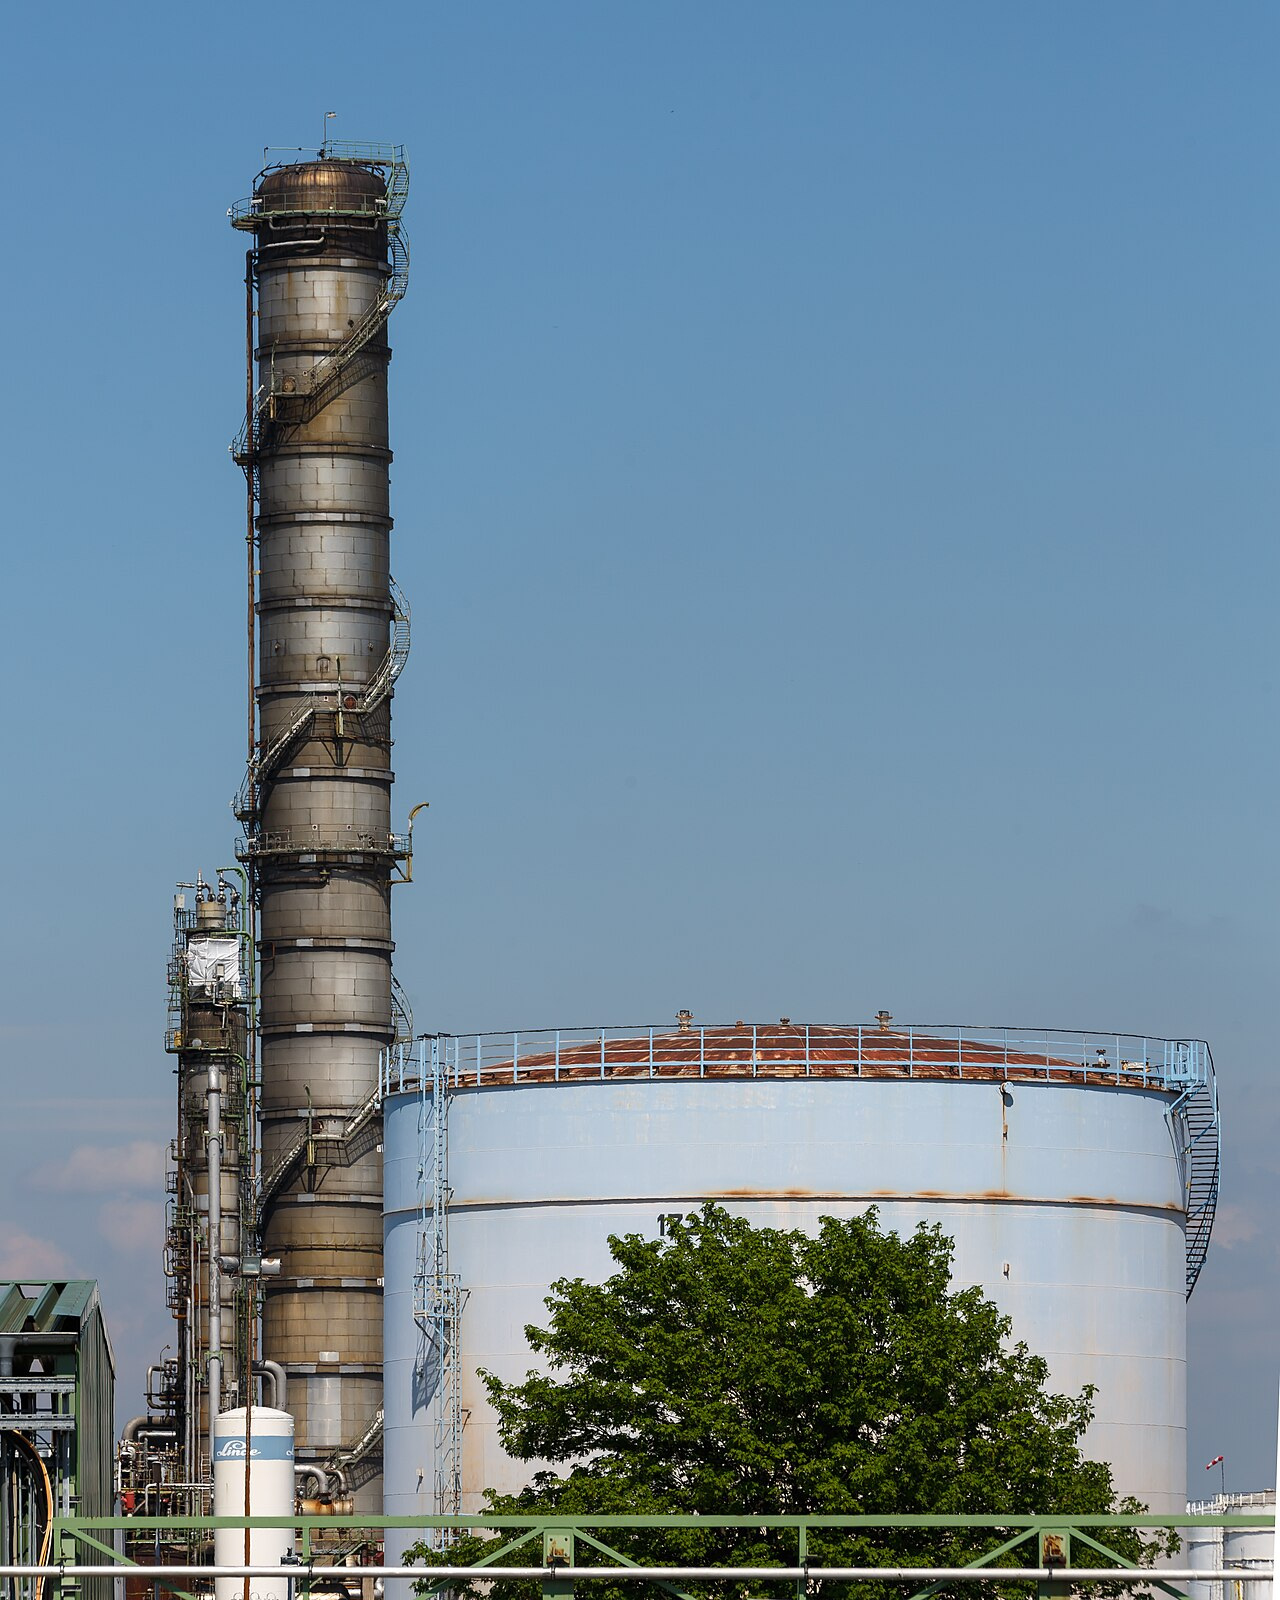
\includegraphics[width=\linewidth]{images/book3/refinery-column.jpg}
\end{minipage}

{\small A la izquierda: una columna de platos. El líquido atraviesa cada plato y baja por
el bajante hasta el plato inferior; el vapor sube a través de los platos y burbujea
a través del líquido. El vapor condensado se devuelve en parte como reflujo; el
hervidor del fondo proporciona el vapor. A la derecha: una columna de destilación de una
refinería (Colonia, 2014), que contiene decenas de platos. (Fotografía: CEphoto,
Uwe Aranas, CC BY-SA 3.0, Wikimedia Commons.)}
\end{omfigure}

\begin{proposition}[Ecuación de Fenske]\label{prop:b2:liquid-vapour-diagrams:fenske}
A reflujo total, con una volatilidad relativa $\alpha$ constante, el número de
\omterm{def:b2:liquid-vapour-diagrams:fractional-distillation}{platos teóricos} necesario para pasar de un líquido de fondo $x_B$ a un destilado
$x_D$ es al menos
\[
  N_{\min} = \frac{1}{\ln\alpha}\,\ln\!\left[\frac{x_D}{1 - x_D}\cdot\frac{1 - x_B}{x_B}\right] .
\]
\end{proposition}

\begin{proof}
Numérense los platos desde abajo, siendo el hervidor el plato 1. A reflujo total
el líquido que baja al plato $k + 1$ tiene la composición del vapor
que sale del plato $k$: $x_{k+1} = y_k$. Con $r = x/(1 - x)$, cada plato da
$r(y_k) = \alpha\,r(x_k)$, luego $r(x_{k+1}) = \alpha\,r(x_k)$, y tras $N$
platos el vapor condensado tiene $r(x_D) = \alpha^N r(x_B)$. Tomando logaritmos
se obtiene $N$. Con un reflujo finito, el líquido que baja es más pobre que el
vapor que sube, cada plato enriquece menos y hacen falta más platos.
\end{proof}

En el diagrama $(x, y)$ la misma construcción es una escalera entre la
curva de equilibrio y la diagonal $y = x$: cada peldaño es un \omterm{def:b2:liquid-vapour-diagrams:fractional-distillation}{plato
teórico}.

\begin{omfigure}
\begin{tikzpicture}
\begin{axis}[width=0.55\linewidth, height=0.55\linewidth, xmin=0, xmax=1,
  ymin=0, ymax=1, axis x line=bottom, axis y line=left,
  xlabel={$x$ (benceno, líquido)}, ylabel={$y$ (benceno, vapor)},
  tick label style={font=\small}, label style={font=\small}]
\addplot[omThm, thick] table[x=x, y=y] {figdata/out/bachelor-2-liquid-vapour-f-eq.dat};
\addplot[black!50] coordinates {(0,0) (1,1)};
\addplot[omDef, thick] table[x=x, y=y] {figdata/out/bachelor-2-liquid-vapour-f.dat};
\draw[densely dotted] (axis cs:0.95,0) -- (axis cs:0.95,0.95);
\draw[densely dotted] (axis cs:0.05,0) -- (axis cs:0.05,0.05);
\node[font=\scriptsize, anchor=south east] at (axis cs:0.945,0.02) {$x_D$};
\node[font=\scriptsize, anchor=south west] at (axis cs:0.05,0.02) {$x_B$};
\end{axis}
\end{tikzpicture}

{\small Platos a reflujo total para benceno--tolueno, a partir de un destilado de
0.95 hacia abajo: cada peldaño horizontal va de un vapor al líquido en
equilibrio con él (un plato), y cada peldaño vertical, de ese líquido al
vapor del plato inferior. Siete peldaños llevan el líquido por debajo de $x_B = 0.05$;
la fórmula de Fenske da 6.5.}
% ledger: antoine:benzene.A, antoine:toluene.A (computed in figdata/bachelor-2/liquid-vapour.py)
\end{omfigure}

\begin{proposition}[Una columna no puede atravesar un azeótropo]\label{prop:b2:liquid-vapour-diagrams:azeotrope-limit}
En una mezcla con \omterm{def:b2:liquid-vapour-diagrams:azeotrope}{azeótropo}, una columna alimentada a un lado de la composición
azeotrópica proporciona como mucho el \omterm{def:b2:liquid-vapour-diagrams:azeotrope}{azeótropo} en un extremo y el componente puro
de ese lado en el otro.
\end{proposition}

\begin{proof}
En el \omterm{def:b2:liquid-vapour-diagrams:azeotrope}{azeótropo} la curva de equilibrio corta la diagonal: $y = x$. Cerca de él
cada peldaño de la escalera se vuelve arbitrariamente pequeño, de modo que ningún número finito de
platos lo alcanza, y ninguno lo atraviesa.
\end{proof}

\begin{method}[Prever una destilación fraccionada]\label{met:b2:liquid-vapour-diagrams:predict-distillation}
\begin{enumerate}
  \item Búsquese el punto de ebullición más bajo accesible desde la alimentación en el
        \omterm{def:b2:liquid-vapour-diagrams:binary-diagram}{diagrama isobárico}: un componente puro o un \omterm{def:b2:liquid-vapour-diagrams:azeotrope}{azeótropo positivo}. Sale
        por la cabeza.
  \item El punto de ebullición más alto del mismo lado (componente puro o
        \omterm{def:b2:liquid-vapour-diagrams:azeotrope}{azeótropo negativo}) queda en el hervidor.
  \item Con un \omterm{def:b2:liquid-vapour-diagrams:azeotrope}{azeótropo}, véase a qué lado de él está la alimentación: solo puede
        obtenerse el componente puro de ese lado.
  \item Para el número de platos, úsese la fórmula de Fenske o la escalera,
        y añádanse platos por el reflujo finito que se use en realidad.
\end{enumerate}
\end{method}

Para etanol y agua alimentados por debajo de 0.881, la cabeza proporciona como mucho el
\omterm{def:b2:liquid-vapour-diagrams:azeotrope}{azeótropo}, y el fondo, agua: ninguna columna da etanol absoluto. Secar el
último tanto por ciento exige otro método: un tamiz molecular que adsorba el agua, o
un tercer componente añadido para romper el \omterm{def:b2:liquid-vapour-diagrams:azeotrope}{azeótropo}.

\begin{omfigure}
\begin{tikzpicture}[font=\small, scale=0.95, >={Stealth}]
  \pic[transform shape] at (0,0) {heatingmantle};
  \pic[transform shape] at (0,0) {rbflask={0.45}{orange!25}};
  \foreach \x/\y in {-0.35/0.25,0.05/0.18,0.35/0.3}
    \fill[black!55] (\x,\y) circle (0.06);
  % Vigreux column from the flask neck (0,3) to (0,6)
  \draw[om glass] (-0.22,3.0) -- (-0.22,6.0) (0.22,3.0) -- (0.22,6.0);
  \foreach \yy in {3.4,3.9,4.4,4.9,5.4} {
    \draw[om glass] (-0.22,\yy) -- (-0.06,\yy+0.18) -- (-0.22,\yy+0.3);
    \draw[om glass] (0.22,\yy+0.15) -- (0.06,\yy+0.33) -- (0.22,\yy+0.45);
  }
  \pic[transform shape] (s) at (0,6.0) {stillhead};
  \pic[transform shape] at ($(s-top)+(0,-0.75)$) {thermometer};
  \pic[transform shape, rotate=-20] (c) at (s-arm) {liebig={3.4}};
  % ground-glass joint between the head's side arm and the condenser
  \draw[om glass, fill=white, rotate around={-20:(s-arm)}] ($(s-arm)+(-0.12,-0.17)$) rectangle ($(s-arm)+(0.14,0.17)$);
  \coordinate (cend) at ($(s-arm)+(-20:3.4)$);
  \pic[transform shape] (a) at (cend) {adapter};
  \pic[transform shape] at ($(a-tip)+(0,-2.4)$) {erlenmeyer={0.22}{orange!12}};
  \draw[<-, omProp, thick] (-0.25,4.6) -- (-1.6,4.6) node[left, text=black,
    align=right] {columna de Vigreux\\ (las indentaciones multiplican\\ los contactos)};
  \draw[<-, omProp, thick] (0.12,6.72) -- (-1.4,7.4) node[left, text=black,
    align=right] {bulbo del termómetro\\ a la altura de la salida lateral};
  \draw[<-, omProp, thick] (1.08,0.3) -- (2.3,-0.2) node[right, text=black]
    {manta calefactora};
  \draw[<-, omProp, thick] ($(a-tip)+(0.75,-2.0)$) -- ++(1.0,0.2)
    node[right, text=black] {destilado};
\end{tikzpicture}

{\small \omterm{def:b2:liquid-vapour-diagrams:fractional-distillation}{Destilación fraccionada} en el laboratorio. Una columna de Vigreux entre
el matraz y la cabeza desempeña el papel de unos pocos \omterm{def:b2:liquid-vapour-diagrams:fractional-distillation}{platos teóricos}: el vapor
se condensa en sus indentaciones y se vuelve a evaporar al subir. La
temperatura en la cabeza se mantiene en el punto de ebullición del componente más volátil
mientras este destila, y luego sube.}
\end{omfigure}

\begin{inthelab}[Separar dos líquidos por destilación fraccionada]
El matraz se llena como mucho hasta la mitad, con piedra pómez, y se calienta suavemente
para que el anillo de vapor que condensa suba lentamente por la columna: una columna
inundada por un calentamiento rápido pierde sus platos. La temperatura de cabeza se anota cada
pocos mililitros; el colector se cambia cuando empieza a subir (se recoge una
\textit{fracción} en cada escalón de temperatura), y el calentamiento se
detiene antes de que el matraz quede seco.
\end{inthelab}

\section{Líquidos parcialmente miscibles e inmiscibles}

\begin{definition}[Laguna de miscibilidad]\label{def:b2:liquid-vapour-diagrams:miscibility-gap}
Una \emph{laguna de miscibilidad}\index{laguna de miscibilidad} es el intervalo de
composiciones globales en el que dos líquidos, a una temperatura dada, se separan en dos
capas líquidas, cada una saturada del otro componente. Un
\emph{heteroazeótropo}\index{heteroazeotropo@heteroazeótropo} es el punto de ebullición de un
líquido de dos capas así: las dos capas líquidas y el vapor coexisten a una
temperatura fija y con una composición del vapor fija.
\end{definition}

En el \omterm{def:b2:liquid-vapour-diagrams:miscibility-gap}{heteroazeótropo} hay dos componentes en tres fases: a presión fija
la \omterm{def:b2:equilibrium-shifts:variance}{varianza} es $2 + 2 - 3 - 1 = 0$. La temperatura se mantiene
constante, como en el punto de ebullición de un líquido puro, mientras quedan
ambas capas.

\begin{omfigure}
\begin{tikzpicture}[font=\small, x=6cm, y=0.08cm]
  \draw[->] (0,0) -- (1.05,0) node[right] {$x$};
  \draw[->] (0,0) -- (0,62) node[above] {$T$};
  \node[below] at (0,0) {2}; \node[below] at (1,0) {1};
  % boiling points: 2 at 50, 1 at 42; heteroazeotrope at 25 with layers 0.1 and 0.85, vapour 0.6
  \draw[omliquidus] (0,50) .. controls (0.04,38) and (0.08,30) .. (0.1,25);
  \draw[omliquidus] (1,42) .. controls (0.95,34) and (0.9,28) .. (0.85,25);
  \draw[omsolidus] (0,50) .. controls (0.25,46) and (0.5,35) .. (0.6,25);
  \draw[omsolidus] (1,42) .. controls (0.9,37) and (0.7,30) .. (0.6,25);
  \draw[thick] (0.1,25) -- (0.85,25);
  \draw[omliquidus] (0.1,25) -- (0.07,2);
  \draw[omliquidus] (0.85,25) -- (0.9,2);
  \fill (0.6,25) circle[radius=2pt];
  \node[font=\scriptsize] at (0.47,6) {dos capas líquidas};
  \node[font=\scriptsize] at (0.5,55) {vapor};
  \node[font=\scriptsize] at (0.035,12) {L$_2$};
  \node[font=\scriptsize] at (0.96,12) {L$_1$};
  \node[font=\scriptsize, align=center] at (0.3,33) {L$_2$ + V};
  \node[font=\scriptsize, anchor=west] at (1.06,36) {L$_1$ + V};
  \draw[thin] (1.06,36) -- (0.86,29.5);
  \node[font=\scriptsize, anchor=north] at (0.6,24) {heteroazeótropo};
\end{tikzpicture}

{\small \omterm{def:b2:liquid-vapour-diagrams:binary-diagram}{Diagrama isobárico} esquemático de dos líquidos parcialmente miscibles. Por debajo de la
temperatura del \omterm{def:b2:liquid-vapour-diagrams:miscibility-gap}{heteroazeótropo} el líquido se separa en dos capas L$_1$ y
L$_2$ en un amplio intervalo de composiciones (la \omterm{def:b2:liquid-vapour-diagrams:miscibility-gap}{laguna de miscibilidad}); sobre la
recta horizontal las dos capas hierven juntas dando un vapor de composición
fija (punto).}
\end{omfigure}

\begin{definition}[Destilación por arrastre de vapor]\label{def:b2:liquid-vapour-diagrams:steam-distillation}
La \emph{destilación por arrastre de vapor}\index{destilacion por arrastre de vapor@destilación por arrastre de vapor} es la destilación de un
líquido inmiscible con el agua haciendo pasar vapor de agua a través de él: la mezcla hierve
por debajo del punto de ebullición de ambos líquidos, y el destilado se separa en
dos capas.
\end{definition}

La \omterm{def:b2:liquid-vapour-diagrams:steam-distillation}{destilación por arrastre de vapor} solo se diferencia de la hidrodestilación del volumen escolar
en el modo de aportar el agua: vapor insuflado a través del material, en lugar de
material hervido en agua. La termodinámica es la misma.

\begin{proposition}[Ebullición de dos líquidos inmiscibles]\label{prop:b2:liquid-vapour-diagrams:steam}
Dos líquidos inmiscibles en contacto hierven a la temperatura a la que la suma de
sus presiones de vapor es igual a la presión exterior, $p_1^*(T) + p_2^*(T) =
p$, inferior a ambos puntos de ebullición. El destilado contiene los dos líquidos
en la razón de masas
\[
  \frac{m_1}{m_2} = \frac{p_1^*\,M_1}{p_2^*\,M_2} .
\]
\end{proposition}

\begin{proof}
Cada líquido puro ejerce su propia presión de vapor, sea cual sea la cantidad del
otro: la presión total sobre las dos capas es $p_1^* + p_2^*$, que
alcanza $p$ a una temperatura a la que cada $p_i^*$ es menor que $p$. En el
vapor las cantidades son proporcionales a las presiones parciales, $n_1/n_2 =
p_1^*/p_2^*$; se multiplica por $M_1/M_2$.
\end{proof}

\begin{omfigure}
\begin{tikzpicture}
\begin{axis}[width=0.6\linewidth, height=5.5cm, xmin=70, xmax=100, ymin=0, ymax=1.6,
  axis x line=bottom, axis y line=left, xlabel={$T$ (\unit{\degreeCelsius})},
  ylabel={$p$ (\unit{bar})}, tick label style={font=\small},
  label style={font=\small}, clip=false]
\addplot[omProp, thick] table[x=t, y=ptol] {figdata/out/bachelor-2-liquid-vapour-e.dat};
\addplot[omDef, thick] table[x=t, y=pwat] {figdata/out/bachelor-2-liquid-vapour-e.dat};
\addplot[black, very thick] table[x=t, y=psum] {figdata/out/bachelor-2-liquid-vapour-e.dat};
\draw[densely dashed] (axis cs:70,1.013) -- (axis cs:100,1.013) node[right, font=\scriptsize] {\qty{1.013}{bar}};
\draw[densely dotted] (axis cs:84.3,0) -- (axis cs:84.3,1.013);
\node[font=\scriptsize, anchor=south east] at (axis cs:84.3,1.05) {\qty{84.3}{\degreeCelsius}};
\node[font=\scriptsize, anchor=west] at (axis cs:96,1.45) {suma};
\node[font=\scriptsize, omDef, anchor=south] at (axis cs:77,0.46) {agua};
\node[font=\scriptsize, omProp, anchor=north west] at (axis cs:88,0.5) {tolueno};
\end{axis}
\end{tikzpicture}

{\small Tolueno y agua, inmiscibles: las presiones de vapor de cada líquido y
su suma. Las dos capas hierven juntas a \qty{84.3}{\degreeCelsius}, por debajo del
agua (\qty{100}{\degreeCelsius}) y del tolueno (\qty{110.6}{\degreeCelsius});
el destilado arrastra 4.1 g de tolueno por gramo de agua.}
% ledger: antoine:toluene.A, antoine:water.A, aw:C, aw:H, aw:O (computed in figdata/bachelor-2/liquid-vapour.py)
\end{omfigure}

Las moléculas pesadas y frágiles de las esencias vegetales destilan así algo
por debajo de \qty{100}{\degreeCelsius}, muy por debajo de sus propios puntos de ebullición, con
poca descomposición; el precio es un destilado que es sobre todo agua.

\section{Ejercicios}

\begin{exercise}[$\star$]\label{exo:b2:liquid-vapour-diagrams:1}
En el \omterm{def:b2:liquid-vapour-diagrams:binary-diagram}{diagrama isobárico} benceno--tolueno, léanse los puntos de ebullición de los líquidos
puros, el \omterm{def:b2:liquid-vapour-diagrams:bubble-dew}{punto de burbuja} de un líquido de composición 0.2 y la composición de
su primer vapor.
\end{exercise}

\begin{exercise}[$\star$]\label{exo:b2:liquid-vapour-diagrams:2}
A \qty{80}{\degreeCelsius} las presiones de vapor del benceno y del tolueno son
\qty{1.010}{bar} y \qty{0.388}{bar}. Calcúlense, para un líquido equimolar, la
presión a la que empieza a hervir y la composición del vapor.
\end{exercise}

\begin{exercise}[$\star$]\label{exo:b2:liquid-vapour-diagrams:3}
\qty{10}{mol} de una mezcla de composición global 0.30 están a una temperatura
a la que el líquido tiene composición 0.20 y el vapor 0.45. Calcúlense las cantidades
de cada fase.
\end{exercise}

\begin{exercise}[$\star$]\label{exo:b2:liquid-vapour-diagrams:4}
Calcúlese la \omterm{def:b2:equilibrium-shifts:variance}{varianza} de una mezcla de benceno--tolueno (a) toda líquida; (b)
en ebullición; (c) en un \omterm{def:b2:liquid-vapour-diagrams:azeotrope}{azeótropo}, para un par que lo tenga, a presión fija.
\end{exercise}

\begin{exercise}[$\star\star$]\label{exo:b2:liquid-vapour-diagrams:5}
Hállese por tanteo el \omterm{def:b2:liquid-vapour-diagrams:bubble-dew}{punto de rocío} de un vapor de benceno--tolueno de composición 0.30 a
\qty{1.013}{bar}, con $p^*_{\text{benceno}}$ y $p^*_{\text{tolueno}}$
(\unit{bar}): 1.80 y 0.742 a \qty{100}{\degreeCelsius}, 2.057 y 0.861 a
\qty{105}{\degreeCelsius}. Dese la composición de la primera gota.
\end{exercise}

\begin{exercise}[$\star\star$]\label{exo:b2:liquid-vapour-diagrams:6}
Una mezcla equimolar de benceno--tolueno se destila de forma simple (sin columna). ¿Cuál es
la composición de las primeras gotas de destilado? ¿Cómo cambian la temperatura y
la composición del destilado a medida que avanza la destilación? ¿Por qué es
mala la separación?
\end{exercise}

\begin{exercise}[$\star\star$]\label{exo:b2:liquid-vapour-diagrams:7}
Un vino de fracción molar 0.05 en etanol se destila de forma fraccionada con una columna muy
eficaz. ¿Qué sale por la cabeza y qué queda en el hervidor?
La misma pregunta para una mezcla de fracción molar 0.95.
\end{exercise}

\begin{exercise}[$\star\star$]\label{exo:b2:liquid-vapour-diagrams:8}
Un componente de una esencia vegetal (masa molar \qty{136}{g/mol}) tiene una presión
de vapor de \qty{0.10}{bar} hacia \qty{97}{\degreeCelsius}, donde la del agua es
\qty{0.91}{bar} (datos del ejercicio). ¿A qué temperatura transcurre la \omterm{def:b2:liquid-vapour-diagrams:steam-distillation}{destilación por arrastre
de vapor} bajo \qty{1.013}{bar}, y cuántos gramos de esencia se
recogen por gramo de agua?
\end{exercise}

\begin{exercise}[$\star\star$]\label{exo:b2:liquid-vapour-diagrams:9}
En el diagrama esquemático de los líquidos parcialmente miscibles, descríbase qué ocurre
cuando una mezcla de dos capas de composición global 0.4 se calienta desde la temperatura
ambiente hasta que está toda vaporizada: fases, temperaturas y composición
del primer vapor.
\end{exercise}

\begin{exercise}[$\star\star\star$]\label{exo:b2:liquid-vapour-diagrams:10}
Con $\alpha = 2.47$, calcúlese el número mínimo de \omterm{def:b2:liquid-vapour-diagrams:fractional-distillation}{platos teóricos} para un
destilado de 0.99 y un fondo de 0.01. Compárese con los 6.5 necesarios para 0.95
y 0.05, y coméntese el coste de la pureza.
\end{exercise}

\begin{exercise}[$\star\star\star$]\label{exo:b2:liquid-vapour-diagrams:11}
A partir del \omterm{def:b2:liquid-vapour-diagrams:binary-diagram}{diagrama isobárico} del benceno--tolueno y de las ecuaciones de Antoine,
explíquese cómo se obtiene el \omterm{def:b2:liquid-vapour-diagrams:binary-diagram}{diagrama isotermo} a \qty{80}{\degreeCelsius}
y por qué en él el dominio del líquido está arriba.
\end{exercise}

\begin{exercise}[$\star\star\star$]\label{exo:b2:liquid-vapour-diagrams:12}
Partiendo de la relación $d\ln p = (y - x)\,dy/[y(1 - y)]$, demuéstrese que a temperatura
fija la presión total aumenta con $x$ dondequiera que el vapor sea
más rico en el componente 1 que el líquido, y dedúzcase que una \omterm{def:b2:chemical-potential:ideal-mixture}{mezcla ideal} no tiene
\omterm{def:b2:liquid-vapour-diagrams:azeotrope}{azeótropo}.
\end{exercise}

\section{Problema: una columna para benceno y tolueno}

\begin{problem}[{Problema de fin de semana --- el diagrama isobárico del benceno y el
tolueno a partir de las ecuaciones de Antoine, una vaporización súbita y la regla de la palanca, el número
mínimo de platos de una columna a reflujo total y el límite que impone un
azeótropo}]
\label{pb:b2:liquid-vapour-diagrams:1}
Datos: ecuaciones de Antoine, $\log_{10}(p^*/\unit{bar}) = A - B/(T + C)$ con $T$ en
kelvin: benceno $A = 4.01814$, $B = \qty{1203.835}{K}$, $C =
\qty{-53.226}{K}$; tolueno $A = 4.07827$, $B = \qty{1343.943}{K}$, $C =
\qty{-53.773}{K}$. Presión \qty{1.013}{bar}; el benceno y el tolueno forman una \omterm{def:b2:chemical-potential:ideal-mixture}{mezcla
ideal}. El \omterm{def:b2:liquid-vapour-diagrams:azeotrope}{azeótropo} etanol--agua contiene un 95~\% de etanol en masa.
% ledger: antoine:benzene.A, antoine:benzene.B, antoine:benzene.C, antoine:toluene.A, antoine:toluene.B, antoine:toluene.C, azeo:ethanol-water.w

\medskip
\noindent\textbf{Parte I --- El diagrama.}
\begin{enumerate}
  \item Calcúlense los puntos de ebullición del benceno y del tolueno a \qty{1.013}{bar}.
  \item Calcúlense $p_1^*$ y $p_2^*$ a \qty{90}{\degreeCelsius}.
  \item Dedúzcanse las composiciones del líquido y del vapor en equilibrio
        a \qty{90}{\degreeCelsius}.
  \item Lo mismo a \qty{100}{\degreeCelsius} ($p_1^* = \qty{1.800}{bar}$, $p_2^* =
        \qty{0.742}{bar}$).
  \item Esbócese el \omterm{def:b2:liquid-vapour-diagrams:binary-diagram}{diagrama isobárico} a partir de estos cuatro puntos y de los líquidos puros.
  \item Hállese por tanteo, con una precisión de
        \qty{0.5}{\degreeCelsius}, el \omterm{def:b2:liquid-vapour-diagrams:bubble-dew}{punto de burbuja} de un líquido equimolar entre \qty{90}{\degreeCelsius} y
        \qty{95}{\degreeCelsius}.
  \item Calcúlese la \omterm{def:b2:equilibrium-shifts:variance}{varianza} de la mezcla en ebullición y dígase qué significa para
        el diagrama.
\end{enumerate}

\medskip
\noindent\textbf{Parte II --- Una vaporización súbita.}
\begin{enumerate}[resume]
  \item Una alimentación equimolar se calienta a \qty{95}{\degreeCelsius} ($p_1^* =
        \qty{1.569}{bar}$, $p_2^* = \qty{0.636}{bar}$). Calcúlense $x$ e $y$.
  \item Para \qty{100}{mol} de alimentación, calcúlense las cantidades de líquido y de vapor.
  \item Calcúlese la cantidad de benceno en cada fase y compruébese el balance.
  \item ¿Qué fracción del benceno se recupera en el vapor?
  \item ¿Qué ocurre si la vaporización súbita se hace a \qty{100}{\degreeCelsius}?
  \item ¿A qué temperatura queda vaporizada toda la alimentación?
\end{enumerate}

\medskip
\noindent\textbf{Parte III --- La columna.}
\begin{enumerate}[resume]
  \item Defínase la volatilidad relativa $\alpha$ y calcúlese en el punto de
        ebullición del benceno.
  \item Calcúlese en el punto de ebullición del tolueno.
  \item Tómese la media geométrica como valor para toda la columna.
  \item Demuéstrese que en un \omterm{def:b2:liquid-vapour-diagrams:fractional-distillation}{plato teórico} $y/(1 - y) = \alpha\,x/(1 - x)$.
  \item Explíquese por qué, a reflujo total, el líquido que entra en un plato tiene la
        composición del vapor que sale del plato inferior.
  \item Dedúzcase la fórmula de Fenske.
  \item Calcúlese el número mínimo de \omterm{def:b2:liquid-vapour-diagrams:fractional-distillation}{platos teóricos} para un destilado de
        0.95 y un fondo de 0.05.
  \item ¿Por qué se dota a una columna real de más platos?
  \item En la escalera del capítulo, cuéntense los peldaños y compárese.
\end{enumerate}

\medskip
\noindent\textbf{Parte IV --- Un \omterm{def:b2:liquid-vapour-diagrams:azeotrope}{azeótropo}.}
\begin{enumerate}[resume]
  \item Calcúlese la fracción molar de etanol en el \omterm{def:b2:liquid-vapour-diagrams:azeotrope}{azeótropo} etanol--agua.
  \item Una alimentación de 0.10 en etanol entra en una columna de cincuenta platos. ¿Qué sale por
        la cabeza y por el fondo?
  \item Indíquese el número mínimo de \omterm{def:b2:liquid-vapour-diagrams:fractional-distillation}{platos teóricos} necesario para separar
        benceno y tolueno en productos del 95~\%.
\end{enumerate}
\end{problem}
